\documentclass[11pt,a4paper]{article}

\usepackage[utf8]{inputenc}
\usepackage[T1]{fontenc}
\usepackage{lmodern}
\usepackage{CJKutf8}
\usepackage{microtype}
\usepackage{amsmath, amssymb}
\usepackage{mathtools}
\usepackage{booktabs}
\usepackage{array}
\usepackage{tabularx}
\usepackage{multirow}
\usepackage{xcolor}
\usepackage{tikz}
\usepackage{pgfplots}
\pgfplotsset{compat=1.18}
\usetikzlibrary{arrows.meta, positioning, shapes.geometric, fit, backgrounds, calc, patterns}
\usepackage{float}
\usepackage{hyperref}
\usepackage[numbers,sort&compress]{natbib}
\usepackage{geometry}
\usepackage{listings}
\usepackage{enumitem}
\usepackage{titlesec}
\usepackage{abstract}

\geometry{
  top=2.5cm, bottom=2.5cm,
  left=2.5cm, right=2.5cm
}

\hypersetup{
  colorlinks=true,
  linkcolor=blue!60!black,
  citecolor=green!50!black,
  urlcolor=blue!70!black
}

\lstset{
  basicstyle=\small\ttfamily,
  backgroundcolor=\color{gray!10},
  frame=single,
  framesep=4pt,
  breaklines=true,
  columns=fullflexible,
  keepspaces=true,
  xleftmargin=0.5em,
  xrightmargin=0.5em
}

\newcommand{\R}{\mathbb{R}}
\newcommand{\St}{S_t}
\newcommand{\Stp}{S_{t+1}}
\newcommand{\hs}{h_s}

\title{
  \textbf{PLAA: Persistent Latent Affective Architecture}\\[0.4em]
  \large From Additive Residual Injection to Learned Latent Modulation in LLMs
}

\author{
  Xiao Ouyang \textup{(\begin{CJK}{UTF8}{gbsn}欧阳潇\end{CJK})}
}

\date{\today}

\begin{document}

\maketitle
\thispagestyle{empty}

\begin{abstract}
We present PLAA (Persistent Latent Affective Architecture), a framework for modeling
temporally evolving latent trajectories within a frozen pretrained LLM (Qwen3-4B).
PLAA maintains a learnable latent state $\St \in \R^{256}$ that evolves via a GRU
cell, and investigates two families of injection mechanism: (1)~\textbf{additive
gated cross-attention} ($h_s + \mathrm{gate} \cdot e_o$) inserted across layers
16--28, and (2)~\textbf{FiLM/AdaLN modulation}
$\bigl(\mathrm{LN}(h_s)\cdot(1+\mathrm{scale}(S))+\mathrm{shift}(S)\bigr)$.
We demonstrate that additive injection suffers from severe control weakness
($\Delta\mathrm{PPL} = 2.01$ against noise $\mathrm{std} = \pm 19$), confirming
that the transformer residual stream robustly absorbs additive perturbations.
FiLM modulation achieves substantially stronger causal influence
($\Delta\mathrm{PPL} = 11.44$ upon removal), but in the direction of
\emph{disruption}: the modulation degrades language modeling loss, confirming that
multiplicative conditioning genuinely alters the residual stream's computational
pathway---a necessary precondition for latent control, though not yet a beneficial
one. However, a fundamental tension
remains: \textbf{temporal coherence and layer-wise specialization are competing
objectives} under the FiLM architecture. Although gradient subspace decoupling is
achieved (cosine similarity $0.99 \to 0.14$), static modulation patterns dominate
over state-driven dynamic control, indicating that learned modulation is spatial
rather than temporal in character. These findings establish PLAA as a framework for
studying \textbf{residual stream factorization via persistent latent modulation}, and
propose candidate architectural directions---including gated routing and competitive computation---to overcome the identified limitations and achieve true dynamical
latent control in LLMs.
\end{abstract}

\newpage
\setcounter{page}{1}

%------------------------------------------------------------------
\section{Introduction}
%------------------------------------------------------------------

Large language models process all inputs through a uniform residual stream\footnote{Residual stream: the sequence of hidden-state vectors passed additively between transformer layers, serving as the primary information pathway through the network.} in which
each token effectively re-initializes the computational state. This design achieves
remarkable local reasoning but provides no mechanism for persistent internal
state---variables that evolve across tokens and modulate computation accordingly.

\textbf{The problem.} LLMs lack emotional continuity and persistent internal
state. Each token is a computational reset.

\textbf{Key contributions.}

\begin{enumerate}[leftmargin=*, label=\textbf{\arabic*.}]

  \item \textbf{Additive injection bottleneck.}
    Gated cross-attention\footnote{Cross-attention: a mechanism where queries from one representation attend to keys and values from a different representation, enabling information flow between heterogeneous feature spaces.} ($h_s + \mathrm{gate} \cdot e_o$) is causally weak
    ($\Delta\mathrm{PPL}\footnote{Perplexity (PPL): a standard metric for language model quality, defined as $2^{H}$ where $H$ is the cross-entropy loss. Lower values indicate better prediction; differences ($\Delta$PPL) measure causal impact of interventions.} = 2.01$ vs.\ noise $\mathrm{std} = \pm 19$). Transformer
    residual streams naturally absorb additive perturbations.

  \item \textbf{FiLM modulation as causal disruption.}
    AdaLN-style feature modulation
    $\bigl(\mathrm{LN}(h_s)\cdot(1+\mathrm{scale})+\mathrm{shift}\bigr)$ achieves
    $5.7\times$ stronger causal influence ($\Delta\mathrm{PPL} = 11.44$). The effect
    direction is disruptive (removal \emph{improves} LM loss), confirming that
    multiplicative conditioning genuinely alters computation---a necessary but not
    sufficient condition for beneficial latent control.

  \item \textbf{Layer differentiation via symmetry breaking.}
    A layer-wise variance regularization loss ($w_{\mathrm{std}}$ penalty) breaks the
    symmetric gradient path (cosine similarity\footnote{Cosine similarity: the angular similarity between two vectors, $\cos\theta = \mathbf{a}\cdot\mathbf{b}/(|\mathbf{a}||\mathbf{b}|)$. A value of 1 indicates parallel vectors (identical direction), 0 indicates orthogonality.} $0.99 \to 0.14$) and achieves
    measurable layer specialization ($w_{\mathrm{std}}: 0.0055 \to 0.0333$).

  \item \textbf{The temporal--specialization tension.}
    A coupling objective designed to make FiLM output follow state dynamics collapses
    layer specialization, revealing a fundamental architectural tradeoff between
    temporal coherence and structural differentiation.

  \item \textbf{Phase transition taxonomy.}
    We identify three distinct dynamical regimes\footnote{Phase transition: borrowed from statistical physics, denoting a qualitative shift in system behavior as a control parameter crosses a critical threshold.}: Phase~1 (violent exploration,
    $|S|>5$, $dS>5$); Phase~2 (convergent modulation, $|S|\sim 1$--$2$,
    $dS\sim 1$); Phase~3 (structural specialization, $w_{\mathrm{std}}>0.05$ ---
    approached but not yet achieved under this architecture).

\end{enumerate}

%------------------------------------------------------------------
\section{Method}
%------------------------------------------------------------------

\subsection{State Pipeline}

\[
  S_0 \;\to\; \text{each turn:}\quad \mathrm{modulation}(\St) \;\to\; \mathrm{forward} \;\to\; h_t \;\to\; \Stp = \mathrm{GRU}(\St,\, h_t)
\]

\begin{figure}[H]
\centering
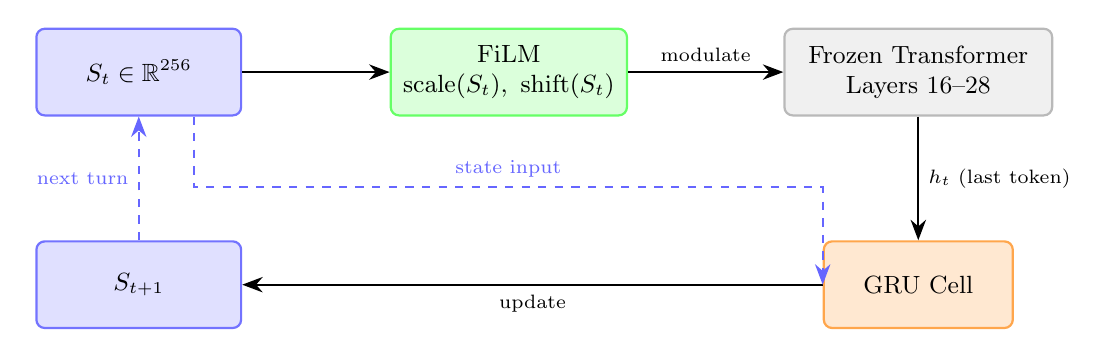
\begin{tikzpicture}[
  font=\small,
  box/.style={rectangle, draw, rounded corners=3pt, minimum height=11mm, align=center, thick},
  state/.style={box, fill=blue!12, draw=blue!55, minimum width=26mm},
  film/.style={box, fill=green!14, draw=green!60, minimum width=30mm},
  tf/.style={box, fill=gray!12, draw=gray!55, minimum width=34mm},
  gru/.style={box, fill=orange!18, draw=orange!70, minimum width=24mm},
  flow/.style={-{Stealth[length=2.6mm]}, thick},
  fb/.style={-{Stealth[length=2.6mm]}, thick, dashed, blue!60}
]
\node[state] (st)   at (0,0)     {$S_t \in \mathbb{R}^{256}$};
\node[film]  (film) at (4.7,0)   {FiLM\\$\mathrm{scale}(S_t),\ \mathrm{shift}(S_t)$};
\node[tf]    (tf)   at (9.9,0)    {Frozen Transformer\\Layers 16--28};
\node[gru]   (gru)  at (9.9,-2.7) {GRU Cell};
\node[state] (stp)  at (0,-2.7)   {$S_{t+1}$};

\draw[flow] (st)   -- (film);
\draw[flow] (film) -- node[above, font=\scriptsize] {modulate} (tf);
\draw[flow] (tf)   -- node[right, font=\scriptsize] {$h_t$ (last token)} (gru);
\draw[flow] (gru)  -- node[below, font=\scriptsize] {update} (stp);
% current state also feeds the GRU as recurrent input
\draw[fb] ($(st.south)+(0.7,0)$) -- ++(0,-0.9)
          -| node[pos=0.25, above, font=\scriptsize] {state input} (gru.west);
% next-turn state becomes the current state (persistence loop)
\draw[fb] (stp) -- node[left, font=\scriptsize] {next turn} (st);
\end{tikzpicture}
\caption{PLAA state pipeline architecture. The latent state $S_t$ drives FiLM modulation of frozen transformer layers; the transformer's output hidden state $h_t$ updates the state via a GRU cell, producing $S_{t+1}$ for the next turn.}
\label{fig:architecture}
\end{figure}

The latent state $\St \in \R^{256}$ evolves via a GRU cell\footnote{Gated Recurrent Unit (GRU)~\cite{cho2014learning}: a recurrent neural network cell that uses update and reset gates to selectively retain or overwrite hidden state across time steps, providing smooth state transitions with fewer parameters than LSTM.} conditioned on the
transformer's final hidden state at the last non-padded token position. The initial
state $S_0$ is a learned parameter with Gaussian noise ($\sigma = 0.01$) for
symmetry breaking.

\subsection{Architecture: Two Injection Mechanisms}

\subsubsection*{Additive Gated Cross-Attention (Phases 1--3B)}

\begin{lstlisting}
Each injected layer:
  Self-Attn -> EmotionCrossAttn(Q=hidden, K,V=e_mem)
            -> GatedResidual(h + gate * eo)
            -> MLP
\end{lstlisting}

\begin{itemize}
  \item $e_{\mathrm{mem}} = \mathrm{proj}(\St) \in \R^{16 \times 2560}$
  \item $\mathrm{gate} \in \R$, initialized $0.1$, with $\tanh$ activation
  \item \textbf{Trainable parameters:} 387M (LoRA\footnote{Low-Rank Adaptation (LoRA)~\cite{hu2022lora}: a parameter-efficient fine-tuning method that injects trainable low-rank decomposition matrices into frozen pretrained weights, drastically reducing the number of trainable parameters while preserving model capacity.} + cross-attention + gate + GRU)
  \item \textbf{Limitation:} the transformer residual absorbs additive signal
\end{itemize}

\subsubsection*{FiLM / AdaLN Modulation (Phase 3C --- primary finding)}

FiLM\footnote{Feature-wise Linear Modulation (FiLM)~\cite{perez2018film}: a conditioning method that applies learned per-channel scale and shift transformations to feature maps. Adaptive Layer Normalization (AdaLN)~\cite{ba2016layer} extends this by applying FiLM-style modulation to layer-normalized activations, enabling external signals to multiplicatively control internal representations.} modulation replaces additive injection with multiplicative feature conditioning:

\begin{lstlisting}
Each injected layer:
  Self-Attn -> AdaLN(LN(hs) * (1 + scale(S)) + shift(S))
            -> MLP
\end{lstlisting}

\begin{itemize}
  \item $\mathrm{scale} = \alpha\cdot\tanh(W_{\mathrm{scale}}\,\St)$,\quad $\mathrm{shift} = \alpha\cdot\tanh(W_{\mathrm{shift}}\,\St)$
  \item $\alpha = 0.1$,\quad $W_{\mathrm{scale}},\, W_{\mathrm{shift}} \in \R^{2560 \times 256}$
  \item \textbf{Trainable parameters:} 17.5M (scale/shift projections + GRU)
  \item \textbf{Result:} $5.7\times$ stronger causal control
\end{itemize}

\subsection{Training Data}

Training uses a 60:30:10 stratified composition across three sources.

\begin{table}[h]
\centering
\begin{tabular}{clll}
\toprule
\textbf{Layer} & \textbf{Ratio} & \textbf{Source} & \textbf{Purpose} \\
\midrule
1 & 60\% & PersonaChat (neutral)      & Latent continuity  \\
2 & 30\% & ESConv (emotional support) & Gradual trajectory \\
3 & 10\% & Bluemoon (RP)              & Dynamic range      \\
\bottomrule
\end{tabular}
\caption{Training data composition.}
\end{table}

\subsection{Optimization}

\begin{itemize}
  \item Frozen Qwen3-4B (4-bit NF4, SDPA)
  \item Trainable: FiLM projections + GRU (17.5M) or LoRA + CA + GRU (387M)
  \item Loss: $\mathcal{W}_{\mathrm{LM}}\cdot\mathcal{L}_{\mathrm{LM}} + \mathcal{W}_{\mathrm{COH}}\cdot\|\Delta S\| + \mathcal{W}_{\mathrm{DIV}}\cdot\mathcal{L}_{\mathrm{repulsion}} + \mathcal{W}_{\mathrm{NORM}}\cdot\|S\|$
  \item Trajectory rollout: 3--5 turn micro-dialogues; GRU rolls along turns
\end{itemize}

%------------------------------------------------------------------
\section{Experiments}
%------------------------------------------------------------------

\subsection{Setup}

\begin{itemize}
  \item \textbf{Model:} Qwen3-4B (4-bit NF4 quantization\footnote{Normal Float 4-bit (NF4): a quantile-based 4-bit data type where quantization levels are optimally spaced for normally distributed weights, enabling aggressive compression with minimal quality degradation.}, SDPA\footnote{Scaled Dot-Product Attention (SDPA): the standard attention computation $\mathrm{softmax}(QK^\top/\sqrt{d_k})V$, here implemented via PyTorch's memory-efficient fused-kernel backend for reduced VRAM usage.} attention, frozen)
  \item \textbf{GPU:} NVIDIA RTX PRO 6000 Blackwell (96\,GB VRAM)
  \item \textbf{Framework:} PEFT\footnote{Parameter-Efficient Fine-Tuning (PEFT): a family of methods (LoRA, adapters, prefix tuning, etc.) that train only a small subset of parameters while keeping the base model frozen, enabling fine-tuning of large models on limited hardware.} (QLoRA\footnote{Quantized LoRA (QLoRA): combines NF4 base-model quantization with LoRA adapters, enabling fine-tuning of models that would otherwise exceed available GPU memory.}) + custom injection layers
  \item \textbf{Key constraint:} Injection \emph{before} PEFT wrapping\\
    Post-wrapping access path: \texttt{peft.base\_model.model.model.layers[i]}
\end{itemize}

\subsection{The Additive Bottleneck}

\subsubsection*{Gate Gradient Diagnostic (Step 1350)}

\begin{lstlisting}
Average gate.grad: 0.056  (non-zero, gradient path EXISTS)
\end{lstlisting}

Despite non-zero gradients, the linear gate ($\text{init}=0.1$, $\tanh$) exhibits
\textbf{multi-stage attenuation}:

\begin{enumerate}
  \item $S_t \approx 0.15$ (norm penalty) $\Rightarrow$ $\mathrm{proj}(S_t)$ small
  \item $\tanh(\mathrm{gate}=0.1) \approx 0.1$
  \item $\times 13$ residual stack $\Rightarrow$ effective influence $\approx 0.0003 \cdot h_{\mathrm{hidden}}$
\end{enumerate}

\subsubsection*{Gate Ablation\footnote{Ablation study: a controlled experiment that removes or disables a specific component to measure its causal contribution to overall system performance.} Test}

\begin{table}[h]
\centering
\begin{tabular}{lcc}
\toprule
\textbf{Condition} & \textbf{PPL} & \textbf{$\Delta$PPL} \\
\midrule
gate $= 0$      & 27.03 & ---  \\
gate $= 1.0$    & 26.26 & 0.77 \\
gate $= 2.0$    & 25.02 & 2.01 \\
gate $=$ random & 25.94 & 1.09 \\
\bottomrule
\end{tabular}
\caption{Gate ablation results. Max $\Delta = 2.01$, noise $\mathrm{std} = \pm 19$.
Causal influence is below the noise floor.}
\end{table}

\textbf{Conclusion:} Additive injection is causally insufficient. The transformer
residual stream absorbs additive perturbations.

\subsection{FiLM Modulation: A Phase Transition}

\subsubsection*{Training Evolution (FiLM v2)}

\begin{table}[h]
\centering
\begin{tabular}{ccccc}
\toprule
\textbf{Step} & \textbf{Loss} & $\boldsymbol{|S|}$ & $\boldsymbol{dS}$ & \textbf{Phase} \\
\midrule
  50 & 45.7 & 9.13 & 5.94 & Phase 1: Violent Exploration \\
 200 & 24.8 & 5.78 & 9.00 & Phase 1 \\
 400 & 14.8 & 1.46 & 1.04 & Phase 2: Transition \\
 600 & 18.5 & 1.15 & 1.34 & Phase 2: Convergence \\
1000 & 15.1 & 0.57 & 0.69 & Phase 2: Stable \\
\bottomrule
\end{tabular}
\caption{FiLM v2 training dynamics.}
\end{table}

\textbf{Phase 1 (steps 1--200):} The latent state dominates computation.
$|S| \sim 5$--$9$, $dS \sim 6$--$10$. The system discovers that latent space can
control computation.

\textbf{Phase 2 (steps 200--1000):} Self-regularization. $|S|$ drops to
$\sim 0.5$--$1.5$, $dS$ to $\sim 0.7$--$1.3$. The system learns selective
modulation. The training dynamics are visualized in Figure~\ref{fig:training-dynamics}.

\begin{figure}[H]
\centering
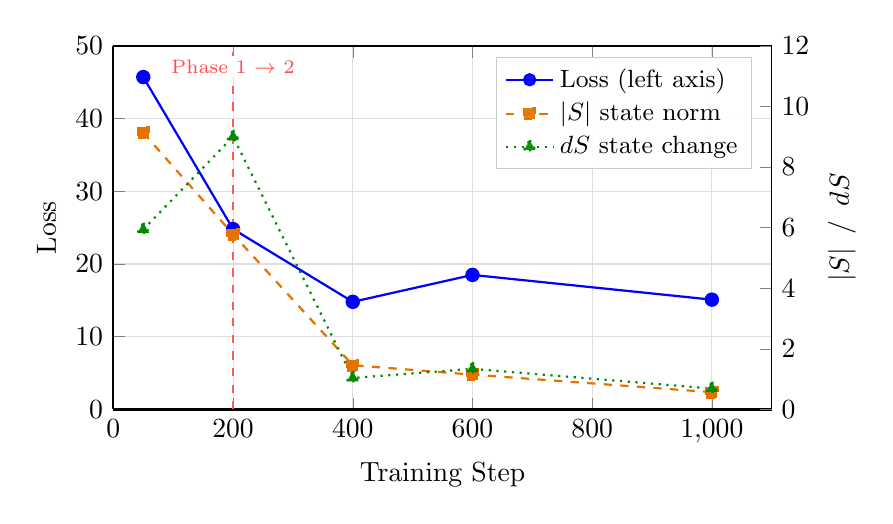
\begin{tikzpicture}
\begin{axis}[
  name=lossaxis,
  width=0.82\linewidth, height=6.2cm,
  xlabel={Training Step}, ylabel={Loss},
  axis y line*=left,
  ymin=0, ymax=50, xmin=0, xmax=1100,
  xtick={0,200,400,600,800,1000},
  ytick={0,10,20,30,40,50},
  grid=major, grid style={gray!25},
  thick,
]
% phase-transition marker
\draw[dashed, red!65, thick] (axis cs:200,0) -- (axis cs:200,50);
\node[font=\scriptsize, red!70, fill=white, inner sep=1.5pt, anchor=south]
  at (axis cs:200,45.5) {Phase 1 $\to$ 2};
\addplot[blue, mark=*, mark size=2.2pt, thick] coordinates {
  (50,45.7) (200,24.8) (400,14.8) (600,18.5) (1000,15.1)};
\end{axis}

\begin{axis}[
  width=0.82\linewidth, height=6.2cm,
  axis y line*=right, axis x line=none,
  ylabel={$|S|$ \,/\, $dS$},
  ymin=0, ymax=12, xmin=0, xmax=1100,
  ytick={0,2,4,6,8,10,12},
  legend style={at={(0.97,0.97)}, anchor=north east, font=\small,
                draw=gray!40, fill=white, fill opacity=0.92, text opacity=1},
  legend cell align=left,
]
% proxy entry so the left-axis Loss curve appears in the combined legend
\addlegendimage{blue, mark=*, thick}\addlegendentry{Loss (left axis)}
\addplot[orange!90!black, mark=square*, mark size=2pt, dashed, thick] coordinates {
  (50,9.13) (200,5.78) (400,1.46) (600,1.15) (1000,0.57)};
\addlegendentry{$|S|$ state norm}
\addplot[green!55!black, mark=triangle*, mark size=2.4pt, dotted, thick] coordinates {
  (50,5.94) (200,9.00) (400,1.04) (600,1.34) (1000,0.69)};
\addlegendentry{$dS$ state change}
\end{axis}
\end{tikzpicture}
\caption{FiLM v2 training dynamics. Phase~1 (steps 1--200) exhibits violent exploration with large state norms and rapid changes. Phase~2 (steps 200--1000) shows convergent self-regularization. The dashed red line marks the phase transition.}
\label{fig:training-dynamics}
\end{figure}

\subsection{Layer Differentiation: Breaking Symmetry}

Adding a layer-wise variance regularization loss
($-0.001 \cdot \mathrm{Var}(\|W_{\mathrm{scale}}\|)$) yields:

\begin{table}[h]
\centering
\begin{tabular}{lcccc}
\toprule
\textbf{Metric} & \textbf{No Diff.\ Loss} & \textbf{With Diff.\ Loss} & \textbf{Target} & \textbf{Status} \\
\midrule
$w_{\mathrm{std}}$   & 0.0055 & \textbf{0.0333} & $>0.05$ & Near threshold \\
grad cosine          & $\sim$0.99 & \textbf{0.11--0.24} & $<0.7$ & \checkmark\ Broken \\
Loss trend           & Stable & Oscillation (14--25) & ---  & Warning \\
\bottomrule
\end{tabular}
\caption{Effect of layer differentiation loss.}
\end{table}

\textbf{Key finding: gradient decoupling $\neq$ parameter specialization.} Cosine
similarity drops from $0.99$ to $0.14$ (layers learn different gradient directions),
but weight norms remain similar. Gradient subspaces have separated, but
parameter-space differentiation lags behind.

\subsection{Causality Test Suite}

\begin{table}[h]
\centering
\begin{tabular}{llcl}
\toprule
\textbf{Test} & \textbf{Loss} & $\boldsymbol{\Delta}$\textsuperscript{$\dagger$} & \textbf{Interpretation} \\
\midrule
Baseline (trained FiLM)        & 14.68 & ---           & Full system \\
FiLM removed ($S=\varnothing$) & 3.14  & \textbf{11.44} & \textbf{Strongly causal (disruptive)} \\
State frozen                   & 13.35 & 1.33          & Weak state coupling \\
\bottomrule
\end{tabular}
\caption{Causality test results. FiLM modulation is strongly causal but disruptive:
removal \emph{lowers} loss, indicating the modulation degrades LM quality while
demonstrating genuine computational influence. The effect is predominantly static
(freezing $S$ changes loss by only 1.33).\\
\textsuperscript{$\dagger$}$\Delta = \mathrm{Loss}_{\mathrm{baseline}} - \mathrm{Loss}_{\mathrm{ablation}}$; positive $\Delta$ means removing the component \emph{lowers} loss (its presence was harmful), negative means removing it raises loss (it was helpful). Here $\Delta = 14.68 - 3.24 \approx +11.44$ confirms FiLM is disruptive.}
\end{table}

\textbf{Critical finding:} FiLM modulation is strongly causal ($\Delta = 11.44$),
but the causal effect is \textbf{static}---freezing $\St$ barely changes output
($\Delta = 1.33$). The system has learned a \textbf{fixed modulation pattern}, not a
state-driven dynamical controller. The contrast between injection mechanisms is shown in Figure~\ref{fig:causal-comparison}.

\begin{figure}[H]
\centering
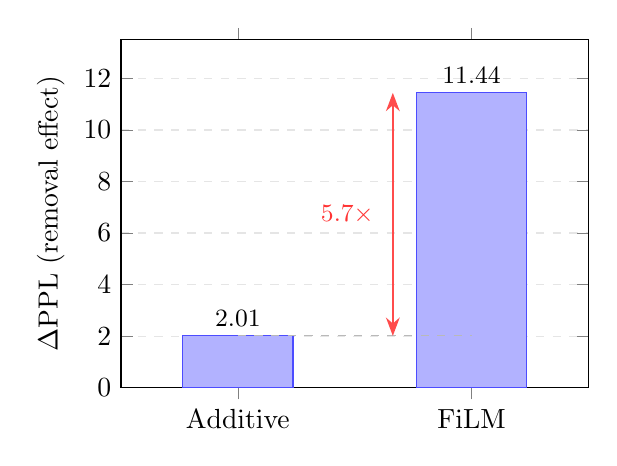
\begin{tikzpicture}
\begin{axis}[
  ybar,
  width=0.62\linewidth, height=6cm,
  ylabel={$\Delta$PPL (removal effect)},
  symbolic x coords={Additive, FiLM},
  xtick=data,
  ymin=0, ymax=13.5,
  ytick={0,2,4,6,8,10,12},
  nodes near coords,
  nodes near coords style={font=\small\bfseries},
  bar width=1.4cm,
  enlarge x limits=0.5,
  ymajorgrids=true,
  grid style={gray!20, dashed},
]
\addplot[fill=blue!30, draw=blue!70] coordinates {
  (Additive, 2.01) (FiLM, 11.44)
};
% reference line at the additive level, and a measured 5.7x gap
\draw[dashed, gray!55] (axis cs:Additive,2.01) -- (axis cs:FiLM,2.01);
\draw[{Stealth}-{Stealth}, thick, red!70]
  ([xshift=-1.0cm]axis cs:FiLM,2.01) -- ([xshift=-1.0cm]axis cs:FiLM,11.44);
\node[anchor=east, text=red!80, font=\small\bfseries]
  at ([xshift=-1.12cm]axis cs:FiLM,6.72) {$5.7\times$};
\end{axis}
\end{tikzpicture}
\caption{Causal influence comparison (ablation $\Delta$PPL). FiLM modulation produces $5.7\times$ stronger effect upon removal ($\Delta\mathrm{PPL} = 11.44$) compared to additive injection ($\Delta\mathrm{PPL} = 2.01$). Note: positive $\Delta$ indicates the component was \emph{increasing} loss---the modulation is disruptive to language modeling but demonstrates genuine computational influence over the residual stream.}
\label{fig:causal-comparison}
\end{figure}

\subsection{The Temporal--Specialization Tension}

Enforcing state-dependent modulation via a coupling loss (maximizing correlation
between $S$ differences and FiLM output differences) reveals a fundamental tradeoff:

\begin{table}[h]
\centering
\begin{tabular}{lccc}
\toprule
\textbf{Variant} & $w_{\mathrm{std}}$ (specialization) & $|S|$ (temporal) & \textbf{cos} \\
\midrule
No coupling (v5)       & \textbf{0.0333} & 0.57 & 0.15 \\
Coupling 0.01 (v6)     & 0.0000          & \textbf{2.59} & 0.19 \\
Coupling 0.001 (v7)    & 0.0000          & 0.44 & 0.16 \\
\bottomrule
\end{tabular}
\caption{Temporal coherence vs.\ layer specialization tradeoff.}
\end{table}

Even at $1/10$ strength, the coupling objective collapses layer specialization
($w_{\mathrm{std}} \to 0$). \textbf{Temporal coherence and structural
specialization are competing objectives in the AdaLN FiLM architecture.}

\subsection{Gate Sensitivity Sweep}

\begin{table}[h]
\centering
\begin{tabular}{cccc}
\toprule
$\boldsymbol{\alpha}$ (tanh bound) & \textbf{Loss} & $w_{\mathrm{std}}$ & $w_{\mathrm{std}}/w_{\mathrm{mean}}$ \\
\midrule
0.05 & 13.98 & 0.0451 & 0.0015 \\
0.10 & 14.08 & 0.0451 & 0.0015 \\
0.20 & 14.03 & 0.0451 & 0.0015 \\
0.30 & 14.31 & 0.0451 & 0.0015 \\
0.50 & 14.56 & 0.0451 & 0.0015 \\
\bottomrule
\end{tabular}
\caption{Complete insensitivity to $\alpha$. The $\tanh$ bound is not the limiting
factor; the modulation structure is intrinsically saturated.
$w_{\mathrm{std}}/w_{\mathrm{mean}} = 0.0015$ is pure initialization noise level.}
\end{table}

%------------------------------------------------------------------
\section{Analysis: Three Findings on Residual Stream Factorization}
%------------------------------------------------------------------

\subsection{Finding 1: Additive Injection is Structurally Weak}

The transformer residual stream is trained from initialization to absorb additive
perturbations. Any signal of the form $h_s + \varepsilon \cdot f(\cdot)$ will be
partially integrated into downstream compensation. Quantitatively:
$\Delta\mathrm{PPL} = 2.01$ vs.\ noise $\mathrm{std} = \pm 19$.

\subsection{Finding 2: Multiplicative Modulation Achieves Causal Disruption}

FiLM achieves $5.7\times$ stronger causal effect than additive injection by changing
feature amplitude directly. However, the direction of this effect is
\emph{disruptive}: removing FiLM \emph{lowers} loss from 14.68 to 3.14, meaning the
modulation degrades language modeling quality. (The 3.14 PPL---dramatically lower than the baseline 14.68---is close to the frozen backbone's native loss without any modulation, confirming that the disruptive effect originates from the FiLM layers rather than from other training artifacts.) The modulation acts on the
\emph{normalized} hidden state, making it much harder for downstream layers to
compensate---which is precisely why it achieves strong causal influence, but also why
it currently imposes a language modeling cost. This establishes that multiplicative
conditioning can genuinely alter the residual stream's computation (unlike additive
injection), but converting this disruptive influence into \emph{beneficial} latent
control remains an open challenge.

\subsection{Finding 3: Static $\gg$ Dynamic in Learned Modulation}

Despite $7000+$ training steps, FiLM modulation is predominantly static. The
coupling between $\St$ and FiLM output is weak (freeze test $\Delta = 1.33$). The
learned parameters $W_{\mathrm{scale}}$ and $W_{\mathrm{shift}}$ have converged to a
fixed modulation pattern that barely varies with $S$, indicating that the system has
learned \emph{which} features to modulate but not \emph{how} to vary that modulation
dynamically.

%------------------------------------------------------------------
\section{Related Work}
%------------------------------------------------------------------

\textbf{Latent state injection.} Prior work on injecting persistent latent states
into LLMs has largely relied on additive gated cross-attention
\cite{sukhbaatar2019augmenting, wu2022memorizing}, which we show is causally
insufficient. Memory-augmented networks \cite{graves2016hybrid} address a related
problem but do not target frozen pretrained transformers.

\textbf{Conditional feature modulation.} FiLM (Feature-wise Linear Modulation)
\cite{perez2018film} and its variants---AdaIN \cite{huang2017arbitrary}, AdaLN
\cite{ba2016layer}, and DiT's conditioning layers \cite{peebles2023scalable}---are
well established in vision but have seen limited study in the LLM residual stream.

\textbf{Residual stream analysis.} Mechanistic interpretability work has shown that
the residual stream acts as a shared communication channel \cite{elhage2021mathematical},
and that layers compose in a largely additive manner. Our findings on additive
injection weakness are consistent with this picture.

%------------------------------------------------------------------
\section{Conclusion \& Future Work}
%------------------------------------------------------------------

\begin{quote}
  \textbf{PLAA's central finding:} LLM residual streams can be factorized via
  persistent latent modulation, but the \emph{nature} of this modulation matters
  fundamentally.
\end{quote}

Additive injection is causally insufficient for meaningful latent control.
Multiplicative FiLM modulation achieves strong causal influence but remains
static---the learned parameters do not produce truly state-dependent dynamics.

The discovered tension between temporal coherence and layer specialization suggests
that achieving full dynamical latent control requires architectural innovations beyond
simple modulation. Candidate directions include \textbf{gated routing mechanisms} or
\textbf{competitive computation} that can naturally differentiate layer roles while
maintaining state-responsiveness.

\subsubsection*{Three-Phase Taxonomy for Latent Dynamics}

\begin{table}[h]
\centering
\begin{tabular}{clcccc}
\toprule
\textbf{Phase} & \textbf{Name} & $|S|$ & $dS$ & $w_{\mathrm{std}}$ & \textbf{cos} \\
\midrule
1 & Violent Exploration    & $>5$        & $>5$         & ---      & ---         \\
2 & Convergent Modulation  & $0.5$--$2$  & $0.5$--$1.5$ & $<0.01$  & $\sim 0.99$ \\
3 & Structural Specialization & $0.3$--$1$ & $0.2$--$0.5$ & $>0.05$ & $<0.3$    \\
\bottomrule
\end{tabular}
\caption{Three-phase taxonomy for latent dynamics. Phase 3 was approached but not
fully achieved under the AdaLN FiLM architecture.}
\end{table}

The phase transition trajectory is visualized in Figure~\ref{fig:phase-diagram}.

\begin{figure}[H]
\centering
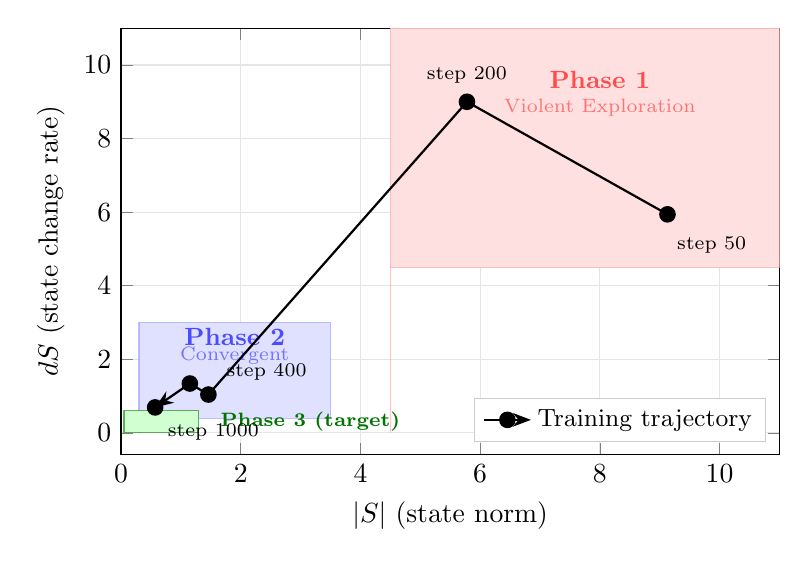
\begin{tikzpicture}
\begin{axis}[
  width=0.82\linewidth, height=7cm,
  xlabel={$|S|$ (state norm)},
  ylabel={$dS$ (state change rate)},
  xmin=0, xmax=11,
  ymin=-0.6, ymax=11,
  xtick={0,2,4,6,8,10}, ytick={0,2,4,6,8,10},
  grid=major, grid style={gray!20},
  legend style={at={(0.98,0.03)}, anchor=south east, font=\small,
                draw=gray!40, fill=white},
  clip=false,
]
% phase regions
\addplot[fill=red!12, draw=red!40, draw opacity=0.6, forget plot]
  coordinates {(4.5,4.5) (11,4.5) (11,11) (4.5,11)} \closedcycle;
\node[font=\small\bfseries, red!70] at (axis cs:8,9.6) {Phase 1};
\node[font=\scriptsize, red!55]     at (axis cs:8,8.85) {Violent Exploration};

\addplot[fill=blue!12, draw=blue!40, draw opacity=0.6, forget plot]
  coordinates {(0.3,0.4) (3.5,0.4) (3.5,3) (0.3,3)} \closedcycle;
\node[font=\small\bfseries, blue!70] at (axis cs:1.9,2.6) {Phase 2};
\node[font=\scriptsize, blue!55]     at (axis cs:1.9,2.1) {Convergent};

\addplot[fill=green!18, draw=green!50!black, draw opacity=0.6, forget plot]
  coordinates {(0.05,0.02) (1.3,0.02) (1.3,0.6) (0.05,0.6)} \closedcycle;
\node[font=\scriptsize\bfseries, green!45!black, anchor=west]
  at (axis cs:1.5,0.3) {Phase 3 (target)};

% training trajectory
\addplot[thick, black, mark=*, mark size=2.6pt, -{Stealth}]
  coordinates {(9.13,5.94) (5.78,9.00) (1.46,1.04) (1.15,1.34) (0.57,0.69)};
\addlegendentry{Training trajectory}

\node[font=\scriptsize, anchor=north west] at (axis cs:9.13,5.6) {step 50};
\node[font=\scriptsize, anchor=south]      at (axis cs:5.78,9.25) {step 200};
\node[font=\scriptsize, anchor=south west] at (axis cs:1.6,1.15) {step 400};
\node[font=\scriptsize, anchor=north west] at (axis cs:0.62,0.5) {step 1000};

\end{axis}
\end{tikzpicture}
\caption{Phase transition diagram in $|S|$--$dS$ space. The training trajectory (black arrows) shows the system transitioning from Phase~1 (violent exploration, high norm and change rate) through Phase~2 (convergent modulation) toward Phase~3 (structural specialization, not fully achieved). Shaded regions indicate the characteristic parameter ranges for each phase.}
\label{fig:phase-diagram}
\end{figure}

%------------------------------------------------------------------
\appendix
%------------------------------------------------------------------

\section{Behavior Divergence Table}

The full 12-cell behavior divergence table documenting qualitative output differences
across injection conditions and state values is provided in the supplementary
materials.

\section{Full Training Pipeline}

\begin{table}[H]
\centering
\begin{tabular}{llccc}
\toprule
\textbf{Phase} & \textbf{Content} & \textbf{Steps} & \textbf{Params} & \textbf{Status} \\
\midrule
1              & YaRN 256K context extension & ---  & ---    & Complete \\
2              & SFT (134K samples)          & ---  & ---    & Complete \\
2.5            & Persona alignment           & ---  & ---    & Complete \\
3A             & Stability validation        & 1K   & ---    & Complete \\
3B             & Gradient flow verification  & ---  & ---    & Complete \\
3C v1          & Single-step additive        & 5K   & 387M   & Complete \\
3C v2          & Trajectory additive         & 1.4K & 387M   & Complete \\
3C v3          & Additive + gate noise       & 6.7K & 387M   & Baseline \\
\textbf{3C FiLM} & \textbf{AdaLN modulation} & \textbf{7K} & \textbf{17.5M} & \textbf{Primary} \\
\bottomrule
\end{tabular}
\caption{Full training pipeline. Dashes (---) in Steps/Params columns indicate phases where these metrics are not applicable (infrastructure setup or validation-only stages).}
\end{table}

\section{Scale/Shift Statistics}

\begin{table}[H]
\centering
\begin{tabular}{lcc}
\toprule
\textbf{Metric} & \textbf{Step 1000} & \textbf{Step 2000} \\
\midrule
scale mean         & 0.0001 & 0.0001 \\
scale std          & 0.0060 & 0.0055 \\
scale max          & 0.0228 & 0.0209 \\
layer\_scale\_std  & 0.0060 & 0.0055 \\
\bottomrule
\end{tabular}
\caption{Scale/shift statistics at steps 1000 and 2000. All 13 layers produce nearly
identical modulation, confirming that no layer specialization is achieved under
baseline AdaLN FiLM training.}
\end{table}

\bibliographystyle{unsrtnat}
\bibliography{references}

\end{document}
